\documentclass[11pt,a4paper]{article}
\usepackage[utf8]{inputenc}
\usepackage[T1]{fontenc}
\usepackage{lmodern}
\usepackage[margin=2.4cm]{geometry}
\usepackage{amsmath,amssymb,booktabs,longtable,array,graphicx,xcolor,listings,tikz}
\usepackage[hidelinks]{hyperref}
\usetikzlibrary{positioning,arrows.meta}
\renewcommand{\contentsname}{Contenido}
\renewcommand{\refname}{Referencias}
\renewcommand{\figurename}{Figura}
\renewcommand{\tablename}{Tabla}
\renewcommand{\abstractname}{Resumen}
\setlength{\parskip}{5pt}
\setlength{\parindent}{0pt}
\setlength{\emergencystretch}{3em}
\lstset{basicstyle=\ttfamily\small,breaklines=true,frame=single,columns=fullflexible,
  keepspaces=true,showstringspaces=false,keywordstyle=\color{blue!55!black},
  commentstyle=\color{green!40!black},numbers=left,numberstyle=\tiny,
  literate={á}{{\'a}}1 {é}{{\'e}}1 {í}{{\'i}}1 {ó}{{\'o}}1 {ú}{{\'u}}1 {ñ}{{\~n}}1}
\newcommand{\code}[1]{\texttt{\detokenize{#1}}}
\newcommand{\miB}{\mathrm{MiB}}
\title{ISAM como método de acceso en PostgreSQL 18.6\\
\large Informe técnico de la Etapa I: bloques internos 0--6}
\author{Grupo 9 -- Bases de Datos II\\[5pt]
\small Medina Grados, Fabian Esteban\\
\small Vargas Llerena, Bryan Aron\\
\small Villanueva Valencia, Andy Jeferson\\
\small Chavez Quijahuaman, Jorge\\
\small Becerra Reymer, Leonardo Sebastian}
\date{Proyecto académico -- 2026-II}
\begin{document}
\maketitle
\begin{abstract}
Se describe una implementación académica de Indexed Sequential Access Method
(ISAM) en C, integrada como Index Access Method de PostgreSQL 18.6. El directorio
estático organiza páginas primarias ordenadas y cadenas de desbordamiento; las
entradas relacionan claves enteras con identificadores de tupla del heap. Se
implementan construcción, igualdad, rango e inserción, y se añaden observabilidad,
reorganización, VACUUM y uso del WAL genérico del DBMS. La validación incluye
pruebas del núcleo, integración SQL, recuperación ante SIGKILL y una regresión
específica de eliminación y VACUUM. La evaluación compara acceso sin índice,
B-tree e ISAM con tres tamaños y cinco repeticiones independientes, empleando
operaciones fijas, semillas y registros verificables. Se separan estos resultados
de los experimentos exploratorios previos y del trabajo distribuido posterior.
\end{abstract}
\tableofcontents
\newpage

\section{Introducción y motivación}
La indexación permite localizar registros sin inspeccionar siempre todas las
páginas de una relación. Su conveniencia depende del costo de construcción,
selectividad, distribución de accesos, espacio y modificaciones de los datos.
El objetivo del proyecto es comprender esas decisiones mediante una estructura
propia y su utilización real desde PostgreSQL, conforme a la propuesta inicial
del equipo~\cite{propuesta} y a las pautas oficiales~\cite{rubrica}.

Se eligió ISAM porque combina una organización secuencial ordenada con un
directorio jerárquico estático y soporta naturalmente igualdad y rango. El diseño
permite observar de forma explícita el compromiso entre un directorio estable y
el costo de las cadenas de overflow. B-tree constituye la referencia del DBMS;
no se plantea que ISAM lo supere en todos los escenarios.

Los objetivos verificables son: construir y consultar un índice propio; insertar
sin perder correspondencia con el heap; ejecutar las operaciones desde el
executor mediante callbacks C; reproducir el entorno; y explicar los resultados
de una comparación controlada. Se adopta clave \code{int4} de una columna, con
duplicados permitidos. No se pretende ofrecer un componente de producción.

\subsection{Alcance y hoja de ruta del equipo}
El informe comprende los bloques internos 0--6. Las etapas oficiales del curso
y los bloques del equipo son organizaciones distintas: el parcial solicita una
implementación integrada y una comparación preliminar; los experimentos
controlados aquí incluidos adelantan la evaluación del índice.

\begin{longtable}{p{0.08\linewidth}p{0.48\linewidth}p{0.32\linewidth}}
\toprule Bloque & Trabajo & Relación con la entrega\\\midrule
0 & Organización del repositorio; separación de núcleo, AM, pruebas y antecedentes & Código actual; \code{legacy/} solo como referencia\\
1 & Docker, PostgreSQL 18.6 y prototipo de AM & Entorno reconstruible y registro del AM\\
2 & Layout, directorio, construcción y búsqueda en C & Núcleo standalone\\
3 & Inserción y overflow & Pruebas y puntero a la cola\\
4 & Callbacks e integración PostgreSQL & Índices reales, scans y bitmap\\
5 & D1/D2/D3, W1--W4 y automatización & Generadores y cuotas reproducibles\\
6 & Comparación y reorganización & Resultados, relleno y REINDEX\\
7 & Fragmentación, asignación y replicación & Pendiente, Etapa II\\
8 & Tres nodos y experimentos distribuidos & Pendiente, Etapa II\\\bottomrule
\end{longtable}

La propuesta declara fuera del alcance mínimo concurrencia completa, WAL propio,
VACUUM especializado y unicidad completa. El uso de mecanismos existentes de
PostgreSQL y las pruebas adicionales se presentan como ampliaciones, sin convertir
esas pruebas en una garantía general de robustez.

\section{Fundamentos teóricos y comparación con B-tree}
ISAM utiliza separadores que se determinan al construir el directorio. Las
inserciones conservan ese directorio y emplean espacio libre en páginas primarias
o páginas de overflow enlazadas. B-tree mantiene una organización dinámica,
mediante divisiones y otras operaciones de mantenimiento. Las referencias
académicas de la propuesta describen este contraste~\cite{ramakrishnan,silberschatz}.

\begin{table}[h]
\centering\small
\begin{tabular}{p{0.22\linewidth}p{0.34\linewidth}p{0.34\linewidth}}
\toprule Aspecto & ISAM implementado & B-tree de referencia\\\midrule
Directorio & Estático entre reconstrucciones & Dinámico\\
Inserción & Espacio primario o overflow & Mantenimiento de páginas y divisiones\\
Búsquedas & Igualdad y rangos por candidatos & Igualdad, rango y capacidades adicionales\\
Degradación & Cadenas largas bajo concentración & Comportamiento condicionado por ocupación y carga\\
Reorganización & Reconstrucción total con REINDEX & Mantenimiento dinámico y REINDEX disponible\\
Capacidades & int4, una columna, sin unicidad ni index-only scan & AM de producción con capacidades más amplias\\\bottomrule
\end{tabular}
\caption{Comparación conceptual; no implica superioridad universal de una alternativa.}
\end{table}

\subsection{Costos temporales, espaciales y de E/S}
Sea $N$ el número de entradas, $f$ el fanout y $h$ la altura del directorio. La
construcción bottom-up sobre entradas ya ordenadas es $O(N)$. El flujo PostgreSQL
recoge y ordena las entradas con \code{qsort}, por lo que debe incluir el costo del
ordenamiento comparativo, del orden de $O(N\log N)$, y memoria $O(N)$. No se debe
atribuir complejidad lineal a toda la operación \code{CREATE INDEX} sobre un heap
no ordenado.

El descenso usa búsqueda binaria dentro de cada página INDEX: $O(h\log f)$
comparaciones. Una consulta debe además inspeccionar las páginas y entradas
candidatas, incluidas sus cadenas; devolver muchos duplicados o un rango amplio
incrementa el costo. El costo de E/S es aproximadamente la altura más las páginas
candidatas y de overflow visitadas. Los límites inferior y superior comparten
lecturas del directorio si recorren una misma rama.

La inserción en una página primaria puede desplazar entradas, con costo acotado
por su capacidad. La cola de overflow evita recorrer toda la cadena para añadir
una entrada; la búsqueda de entradas existentes aún puede visitarla completa.
REINDEX relee el heap, ordena y reconstruye el índice, con costo global y bloqueo
de la operación ordinaria. El espacio crece con $N$ y las páginas de overflow.

\section{Diseño físico y layout en C}
Las páginas tienen 8192 bytes. En modo PostgreSQL se reservan 24 bytes para la
cabecera del DBMS y 16 bytes para \code{IsamBlockHeader}. En modo standalone no
existe la cabecera PostgreSQL. Las constantes y comprobaciones estáticas se
encuentran en \code{isam_am/core/isam_layout.h}.

\begin{figure}[h]
\centering
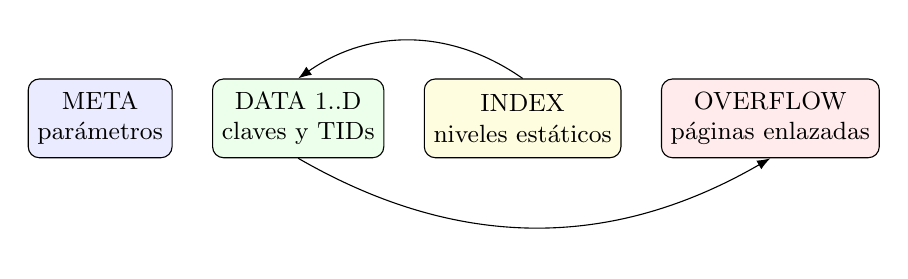
\begin{tikzpicture}[node distance=0.5cm,box/.style={draw,rounded corners,minimum height=1cm,align=center,font=\small},>=Latex]
\node[box,fill=blue!8] (meta) {META\\parámetros};
\node[box,right=of meta,fill=green!8] (data) {DATA 1..D\\claves y TIDs};
\node[box,right=of data,fill=yellow!12] (index) {INDEX\\niveles estáticos};
\node[box,right=of index,fill=red!8] (overflow) {OVERFLOW\\páginas enlazadas};
\draw[->] (index.north) to[bend right=35] (data.north);
\draw[->] (data.south) to[bend right=30] (overflow.south);
\end{tikzpicture}
\caption{Organización física del índice. Las páginas contienen referencias al heap.}
\end{figure}

\begin{itemize}
\item META almacena magic, versión del formato, capacidades, relleno, número de
páginas primarias y niveles, raíz y ubicación de los niveles.
\item DATA almacena entradas primarias ordenadas y el enlace a su cadena.
\item INDEX contiene pares separador--bloque hijo. Los separadores son estáticos.
\item OVERFLOW contiene entradas anexadas y el enlace a la siguiente página;
sus entradas no tienen que estar ordenadas.
\end{itemize}

\code{IsamEntry} ocupa 12 bytes: clave int32, bloque del heap uint32, offset uint16
y dos bytes reservados. \code{IsamIndexEntry} ocupa 8 bytes: clave int32 y bloque
hijo uint32. El TID identifica la ubicación de la tupla, no su valor completo.

\[
C_{DATA,PG}=\left\lfloor\frac{8192-24-16}{12}\right\rfloor=679,
\qquad f_{INDEX,PG}=\left\lfloor\frac{8192-24-16}{8}\right\rfloor=1019.
\]
En standalone las capacidades son 681 y 1022. El factor de llenado inicial,
entre 10 y 100, reserva holgura en DATA; la inserción puede utilizar la capacidad
completa antes de crear overflow. La GUC \code{isam_am.fill_pct} tiene valor
predeterminado 80. El formato utiliza el orden de bytes nativo y no se reclama
portabilidad arbitraria de archivos físicos entre arquitecturas.

\section{Implementación e integración en PostgreSQL}
El AM se registra con \code{CREATE ACCESS METHOD ... TYPE INDEX} y una operator
class int4 para estrategias $<,\le,=,\ge,>$. La interfaz oficial conecta estas
operaciones con \code{IndexAmRoutine}~\cite{postgres}.

\begin{longtable}{p{0.19\linewidth}p{0.25\linewidth}p{0.44\linewidth}}
\toprule Operación & Callback/función & Archivo y responsabilidad\\\midrule
Registro & \code{isam_handler} & \code{isam_handler.c}: capacidades y callbacks\\
Construcción & \code{isam_ambuild} & \code{isam_am_build.c}: leer heap, ordenar, construir\\
Índice inicial & \code{isam_ambuildempty} & Fork INIT para tablas UNLOGGED\\
Inserción & \code{isam_aminsert} & \code{isam_am_insert.c}: convertir clave/TID y serializar\\
Abrir/reiniciar scan & \code{ambeginscan}, \code{amrescan} & \code{isam_am_scan.c}: límites y estado diferido\\
Tuplas/bitmap & \code{amgettuple}, \code{amgetbitmap} & Devolver TIDs al executor\\
Costos & \code{amcostestimate} & \code{genericcostestimate}, aproximación simplificada\\
VACUUM & \code{ambulkdelete}, \code{amvacuumcleanup} & Eliminar entradas muertas y actualizar estadísticas\\
E/S y WAL & \code{isam_write_block} & \code{core/isam_io_pg.c}: buffers y GenericXLog\\
Observabilidad & \code{isam_index_stats} & Contar entradas y cadenas; \code{isam_reorg_needed} evalúa umbral\\\bottomrule
\end{longtable}

El flujo es SQL $\rightarrow$ planner $\rightarrow$ executor $\rightarrow$ callbacks
del AM $\rightarrow$ núcleo ISAM $\rightarrow$ buffer manager. Los TIDs devueltos
permiten que PostgreSQL consulte el heap y aplique su visibilidad MVCC. La
extensión no sustituye el gestor de tuplas del DBMS.

\begin{lstlisting}[language=SQL,caption={Uso del método de acceso real}]
CREATE EXTENSION isam_am;
SET isam_am.fill_pct=80;
CREATE INDEX idx ON tabla USING isam_am(id);
EXPLAIN (ANALYZE, BUFFERS)
  SELECT payload FROM tabla WHERE id=680;
SELECT * FROM isam_index_stats('idx');
SELECT isam_reorg_needed('idx',25);
\end{lstlisting}

La implementación omite NULL en el índice. No soporta unicidad, múltiples
columnas, ordenamiento por índice, scans hacia atrás, index-only scan ni
construcción paralela. No se reclama soporte de CREATE INDEX CONCURRENTLY. Los
insertadores se serializan por el bloqueo de extensión de la relación. El
estimador de costos no incorpora una modelación sofisticada de las cadenas.

\section{Validación funcional, casos extremos y recuperación}
La suite standalone comprueba vacío, igualdad, rangos, límites int32, duplicados,
relleno, overflow, persistencia, eliminación y reparación del puntero de cola.
Después de añadir la regresión de VACUUM ejecutó \textbf{121\,452 verificaciones}
(3774 + 117678), sin fallos.

La integración SQL comprueba diez estados con 21 predicados cada uno:
\textbf{210 comparaciones} contra seqscan, más aserciones y comprobaciones de
planes. Incluye construcción, inserción, UPDATE/DELETE, VACUUM, VACUUM FULL,
REINDEX, relleno 100, UNLOGGED, TEMP e índice creado vacío.

\subsection{Regresión de DELETE y VACUUM y su corrección}
El caso \code{tests/sql/caso-vacuum.sql} construye dos páginas primarias llenas,
inserta otra fila de clave 680 en overflow, borra solamente la original y ejecuta
VACUUM. La versión anterior devolvía una fila por seqscan y cero por ISAM: el
escaneo usaba la primera clave primaria superviviente como si fuera el separador
estático. Al compactar la página, ese mínimo aumentaba, mientras que overflow
conservaba una clave menor.

La corrección conserva VACUUM y modifica el lector. \code{isam_index_range_blocks}
calcula las páginas candidatas a partir de separadores estáticos. El scan usa el
último candidato como condición de finalización, examina el overflow de cada
página visitada y nunca descarta una cadena basándose solo en el mínimo primario
mutable. Los caminos del directorio se comparten cuando es posible.

La regresión exige la fila superviviente antes de REINDEX por Index Scan y Bitmap
Scan, comprueba rangos inclusivos/exclusivos y ausencia, y verifica que REINDEX
mantenga el resultado. El núcleo incorpora el caso equivalente y persistencia.
La igualdad habitual en la prueba de un millón de claves conserva tres lecturas
de bloque; un rango de 10 000 claves conserva las 18 lecturas observadas en esa
prueba, sin atribuir esas lecturas standalone a I/O físico del servidor.

\subsection{SIGKILL y WAL genérico}
Las páginas se escriben mediante GenericXLog: las nuevas utilizan imagen completa
y las existentes deltas. No se implementa un formato de WAL independiente.
\code{make crash} mata el contenedor con SIGKILL, reinicia y comprueba el índice
contra el heap, además de la pérdida esperada de datos UNLOGGED. \code{make crash-load}
inyecta la caída con seis clientes insertando y verifica conteo y suma tras
recuperación. Ambas pruebas pasaron en el entorno Docker 18.6 corregido.

Estas pruebas no demuestran corrección para todos los interleavings ni preservación
de transacciones no confirmadas. Las mediciones históricas de volumen WAL
160--57 MB no se incorporan como resultados nuevos porque los CSV aportados no
incluyen sus logs. Deltas de GenericXLog no equivalen a medir \code{wal_compression}.

\section{Metodología y resultados experimentales}
\subsection{Entorno y diseño controlado}
La imagen utiliza PostgreSQL 18.6 y el commit oficial:\\
\code{724edf9bde9d356724ad384a2e196edc3c9f80f7}. El servidor, herramientas y PGXS
se compilan conjuntamente. La descarga y la imagen base se verifican mediante
SHA-256; los paquetes de compilación mantienen firmas y TLS. La configuración
académica no incluye ICU, readline ni zlib. La versión real y parámetros del
servidor se guardan en los metadatos de cada corrida.

El entorno de esta ejecución tiene un límite cgroup de cuatro CPU equivalentes
y aproximadamente 33 GiB de memoria visible. La afinidad y los límites exactos
se conservan en \code{docs/results/resource-limits.json}; el número de CPU
visible del host no se confunde con la cuota efectiva.

Se desactiva JIT y el paralelismo de consultas para aislar las alternativas; la
construcción fija \code{max_parallel_maintenance_workers=0}. Se mantienen fsync,
confirmación síncrona y WAL de páginas completas según los valores registrados.
Las operaciones se ejecutan con hasta cuatro clientes y un hilo por cliente.
La latencia de pgbench es la media dentro de cada réplica; las tablas resumen
la mediana de esas medias, no un percentil de latencias individuales.

Los datos se recargan antes de cada alternativa y repetición. Se validan cantidad,
unicidad y dominio y se ejecuta VACUUM ANALYZE. Este procedimiento implica datos
leídos previamente; no se presenta como un experimento de caché fría. La política
es igual para las alternativas. Los scripts bloquean operaciones concurrentes
de demo/recuperación sobre el contenedor durante la medición.

\subsection{Datasets y cargas}
\begin{table}[h]\centering\small
\begin{tabular}{p{0.1\linewidth}p{0.52\linewidth}p{0.27\linewidth}}
\toprule ID & Definición & Tamaños\\\midrule
D1 & Claves únicas 1..N, carga secuencial & 100k, 500k, 1M\\
D2 & Permutación aleatoria única de 1..N, semilla SQL 0.42 & 100k, 500k, 1M\\
D3 & Exactamente los datos D2; consultas Zipf con parámetro 1.1 & 100k, 500k, 1M\\\bottomrule
\end{tabular}\caption{Definiciones alineadas con la rúbrica; distribución de accesos y de valores se distinguen.}
\end{table}
La unicidad D2 se obtiene por construcción, sin muestreo con reemplazo. D3 incluye
\code{d2.sql}; el sesgo se aplica al elegir claves de consulta, no al duplicar
filas. D4/D5 y búsquedas por prefijo quedan fuera del alcance int4 de la propuesta.

\begin{table}[h]\centering\small
\begin{tabular}{p{.12\linewidth}p{.57\linewidth}p{.23\linewidth}}\toprule Carga & Operación & Cuota por réplica\\\midrule
W1 & Igualdad sobre claves existentes & 10 000 consultas\\
W2 & Igualdad sobre claves ausentes en (N,2N] & 10 000 consultas\\
W3 & Inserción uniforme de claves del dominio, duplicados permitidos & N/10 filas\\
W4 & Rango inclusivo de amplitud floor(N/1000) & 1 000 consultas\\
Posteriores & Repetir W1 y W4 tras W3 & 10 000 y 1 000 consultas\\\bottomrule
\end{tabular}\caption{Operaciones fijas; W3 aumenta la cantidad de filas exactamente un 10\%.}
\end{table}

Cada medición tiene cinco repeticiones independientes. En cada réplica se vuelve
a medir CREATE INDEX; el tiempo no se copia de una construcción anterior. La
semilla pgbench es 42000 + número de réplica, idéntica entre alternativas. Cada
cliente ejecuta una cuota fija mediante \code{-t}; no se usan duraciones fijas
que produzcan cantidades distintas de inserciones. Se verifica el conteo final
y la huella del multiconjunto insertado. La independencia es del estado de cada
corrida; no presupone independencia estadística absoluta respecto de cachés o
variaciones del host.

En el barrido principal W3 utiliza una transacción por fila insertada. Los
tamaños físicos se convierten a MiB, donde $1\,\mathrm{MiB}=2^{20}$ bytes.

Las consultas agregan \code{payload} para requerir acceso al heap. Esta decisión
controla una comparación específica; excluye deliberadamente la ventaja de
index-only scan disponible en ciertos usos de B-tree y no representa todos sus
casos de aplicación. El planner puede elegir su plan; los benchmarks no fuerzan
ISAM. Los buffers registrados corresponden a predicados de muestra, no al
promedio de todas las consultas ni directamente a lecturas físicas.

\subsection{Resultados corregidos y dispersión}
Los resultados se importan del CSV corregido y de sus metadatos con estado
\code{completed}. El generador de tablas rechaza una cuadrícula incompleta,
transacciones fallidas o cuotas incorrectas. Se reporta mediana y rango
intercuartílico (IQR) entre las cinco réplicas. El IQR es una medida descriptiva,
no un intervalo de confianza ni una prueba de equivalencia estadística.

% BEGIN GENERATED BENCHMARK
La corrida verificada contiene 810 observaciones, 135 cargas independientes y 90 construcciones de índices. El IQR se indica entre corchetes. Todos los conteos y huellas entre alternativas fueron verificados.

Versión registrada: PostgreSQL 18.6 on x86\_64-pc-linux-gnu, compiled by gcc (Debian 14.2.0-19) 14.2.0, 64-bit.\par

\begin{table}[htbp]
\centering\small
\caption{Construcción (ms): mediana [IQR], y tamaño inicial (MiB).}\label{tab:build}
\resizebox{\linewidth}{!}{%
\begin{tabular}{lrrrrr}
\toprule
Datos & N & B-tree ms & ISAM ms & B-tree MiB & ISAM MiB \\
\midrule
D1 & 100\,000 & 24.000 [3.511] & 11.588 [1.244] & 2.16 & 1.46 \\
D1 & 500\,000 & 91.447 [10.039] & 47.667 [2.815] & 10.73 & 7.21 \\
D1 & 1\,000\,000 & 172.407 [5.425] & 94.946 [2.221] & 21.45 & 14.42 \\
D2 & 100\,000 & 30.099 [1.952] & 22.221 [0.363] & 2.16 & 1.46 \\
D2 & 500\,000 & 168.088 [29.991] & 114.604 [6.054] & 10.73 & 7.21 \\
D2 & 1\,000\,000 & 411.475 [34.180] & 235.824 [8.886] & 21.45 & 14.42 \\
D3 & 100\,000 & 29.738 [1.553] & 23.789 [1.163] & 2.16 & 1.46 \\
D3 & 500\,000 & 169.060 [23.696] & 114.744 [1.551] & 10.73 & 7.21 \\
D3 & 1\,000\,000 & 439.200 [149.195] & 243.502 [13.298] & 21.45 & 14.42 \\
\bottomrule
\end{tabular}}
\end{table}

\begin{table}[htbp]
\centering\small
\caption{Igualdad exitosa W1: TPS y latencia media por réplica (ms), resumidos con mediana [IQR].}\label{tab:w1_eq_uniform}
\resizebox{\linewidth}{!}{%
\begin{tabular}{lrrrrrrr}
\toprule
Datos & N & Sin TPS & B-tree TPS & ISAM TPS & Sin ms & B-tree ms & ISAM ms \\
\midrule
D1 & 100\,000 & 1294 [32] & 44475 [3807] & 60563 [14290] & 3.090 [0.078] & 0.090 [0.007] & 0.066 [0.018] \\
D1 & 500\,000 & 231 [6] & 46510 [9759] & 47825 [1752] & 17.294 [0.447] & 0.086 [0.017] & 0.084 [0.004] \\
D1 & 1\,000\,000 & 113 [0] & 40737 [6193] & 43941 [3986] & 35.261 [0.146] & 0.098 [0.014] & 0.091 [0.008] \\
D2 & 100\,000 & 1293 [53] & 46838 [4047] & 50871 [3313] & 3.093 [0.128] & 0.085 [0.007] & 0.079 [0.005] \\
D2 & 500\,000 & 238 [7] & 47625 [6192] & 51102 [14941] & 16.802 [0.475] & 0.084 [0.011] & 0.078 [0.026] \\
D2 & 1\,000\,000 & 112 [1] & 44296 [8910] & 46604 [6655] & 35.661 [0.461] & 0.090 [0.016] & 0.086 [0.011] \\
D3 & 100\,000 & 1309 [56] & 48374 [12018] & 47202 [6748] & 3.056 [0.126] & 0.083 [0.020] & 0.085 [0.011] \\
D3 & 500\,000 & 234 [10] & 40685 [11400] & 48216 [4895] & 17.124 [0.793] & 0.098 [0.022] & 0.083 [0.009] \\
D3 & 1\,000\,000 & 113 [5] & 40830 [7067] & 48916 [6131] & 35.302 [1.502] & 0.098 [0.014] & 0.082 [0.011] \\
\bottomrule
\end{tabular}}
\end{table}

\begin{table}[htbp]
\centering\small
\caption{Igualdad ausente W2: TPS y latencia media por réplica (ms), resumidos con mediana [IQR].}\label{tab:w2_eq_absent}
\resizebox{\linewidth}{!}{%
\begin{tabular}{lrrrrrrr}
\toprule
Datos & N & Sin TPS & B-tree TPS & ISAM TPS & Sin ms & B-tree ms & ISAM ms \\
\midrule
D1 & 100\,000 & 1297 [30] & 57594 [7668] & 52896 [15054] & 3.085 [0.072] & 0.069 [0.010] & 0.076 [0.019] \\
D1 & 500\,000 & 235 [8] & 60508 [11393] & 47604 [563] & 17.057 [0.638] & 0.066 [0.015] & 0.084 [0.001] \\
D1 & 1\,000\,000 & 115 [3] & 50198 [14630] & 48665 [3857] & 34.675 [0.946] & 0.080 [0.019] & 0.082 [0.006] \\
D2 & 100\,000 & 1282 [49] & 58058 [11251] & 54680 [7145] & 3.120 [0.117] & 0.069 [0.013] & 0.073 [0.010] \\
D2 & 500\,000 & 235 [3] & 51808 [9671] & 46983 [4646] & 16.986 [0.212] & 0.077 [0.014] & 0.085 [0.008] \\
D2 & 1\,000\,000 & 113 [6] & 46799 [4304] & 49234 [6397] & 35.276 [1.935] & 0.085 [0.008] & 0.081 [0.011] \\
D3 & 100\,000 & 1293 [45] & 47893 [9921] & 54561 [3910] & 3.094 [0.105] & 0.084 [0.015] & 0.073 [0.005] \\
D3 & 500\,000 & 229 [8] & 59343 [2678] & 56849 [5780] & 17.492 [0.604] & 0.067 [0.003] & 0.070 [0.008] \\
D3 & 1\,000\,000 & 111 [1] & 49127 [10285] & 48417 [4287] & 36.064 [0.200] & 0.081 [0.019] & 0.083 [0.008] \\
\bottomrule
\end{tabular}}
\end{table}

\begin{table}[htbp]
\centering\small
\caption{Rango W4: TPS y latencia media por réplica (ms), resumidos con mediana [IQR].}\label{tab:w4_range}
\resizebox{\linewidth}{!}{%
\begin{tabular}{lrrrrrrr}
\toprule
Datos & N & Sin TPS & B-tree TPS & ISAM TPS & Sin ms & B-tree ms & ISAM ms \\
\midrule
D1 & 100\,000 & 1140 [54] & 33228 [3316] & 30983 [3141] & 3.510 [0.163] & 0.120 [0.013] & 0.129 [0.012] \\
D1 & 500\,000 & 217 [4] & 20868 [1110] & 22241 [580] & 18.433 [0.375] & 0.192 [0.010] & 0.180 [0.005] \\
D1 & 1\,000\,000 & 111 [4] & 16900 [1450] & 14930 [2923] & 36.171 [1.346] & 0.237 [0.021] & 0.268 [0.053] \\
D2 & 100\,000 & 1076 [66] & 20245 [4650] & 22681 [2123] & 3.718 [0.223] & 0.198 [0.038] & 0.176 [0.018] \\
D2 & 500\,000 & 204 [5] & 8286 [837] & 7926 [575] & 19.641 [0.512] & 0.483 [0.049] & 0.505 [0.037] \\
D2 & 1\,000\,000 & 98 [6] & 4250 [471] & 4294 [327] & 40.861 [2.541] & 0.941 [0.098] & 0.931 [0.075] \\
D3 & 100\,000 & 1112 [67] & 21568 [1977] & 22506 [5215] & 3.598 [0.213] & 0.185 [0.018] & 0.178 [0.040] \\
D3 & 500\,000 & 202 [2] & 9163 [1126] & 10037 [1288] & 19.817 [0.208] & 0.437 [0.059] & 0.399 [0.055] \\
D3 & 1\,000\,000 & 97 [5] & 4958 [900] & 5064 [107] & 41.383 [2.049] & 0.807 [0.140] & 0.790 [0.017] \\
\bottomrule
\end{tabular}}
\end{table}

\begin{table}[htbp]
\centering\small
\caption{Inserción W3: TPS y latencia media por réplica (ms), resumidos con mediana [IQR].}\label{tab:w3_insert}
\resizebox{\linewidth}{!}{%
\begin{tabular}{lrrrrrrr}
\toprule
Datos & N & Sin TPS & B-tree TPS & ISAM TPS & Sin ms & B-tree ms & ISAM ms \\
\midrule
D1 & 100\,000 & 9792 [699] & 9750 [259] & 9159 [1218] & 0.408 [0.030] & 0.410 [0.010] & 0.437 [0.055] \\
D1 & 500\,000 & 10087 [222] & 9681 [201] & 9636 [96] & 0.397 [0.009] & 0.413 [0.008] & 0.415 [0.004] \\
D1 & 1\,000\,000 & 10054 [659] & 9700 [680] & 9206 [706] & 0.398 [0.026] & 0.412 [0.030] & 0.435 [0.032] \\
D2 & 100\,000 & 10097 [776] & 9980 [444] & 8838 [578] & 0.396 [0.029] & 0.401 [0.017] & 0.453 [0.029] \\
D2 & 500\,000 & 9803 [619] & 10239 [282] & 10098 [348] & 0.408 [0.025] & 0.391 [0.011] & 0.396 [0.014] \\
D2 & 1\,000\,000 & 9957 [419] & 9919 [688] & 9451 [347] & 0.402 [0.017] & 0.403 [0.029] & 0.423 [0.015] \\
D3 & 100\,000 & 10664 [572] & 10539 [3165] & 9426 [500] & 0.375 [0.021] & 0.380 [0.161] & 0.424 [0.021] \\
D3 & 500\,000 & 10404 [366] & 9921 [596] & 9803 [698] & 0.384 [0.014] & 0.403 [0.025] & 0.408 [0.030] \\
D3 & 1\,000\,000 & 9830 [438] & 10103 [420] & 9636 [89] & 0.407 [0.018] & 0.396 [0.017] & 0.415 [0.004] \\
\bottomrule
\end{tabular}}
\end{table}

\begin{table}[htbp]
\centering\small
\caption{Estado después de insertar exactamente un 10\% de filas; tamaños en MiB.}\label{tab:after}
\resizebox{\linewidth}{!}{%
\begin{tabular}{lrrrrrr}
\toprule
Datos & N inicial & Filas finales & B-tree MiB & ISAM MiB & Overflow ISAM & Cadena ISAM \\
\midrule
D1 & 100\,000 & 110000 & 2.17 & 1.46 & 0 [0] & 0 [0] \\
D1 & 500\,000 & 550000 & 10.80 & 7.21 & 0 [0] & 0 [0] \\
D1 & 1\,000\,000 & 1100000 & 21.60 & 14.42 & 0 [0] & 0 [0] \\
D2 & 100\,000 & 110000 & 2.17 & 1.46 & 0 [0] & 0 [0] \\
D2 & 500\,000 & 550000 & 10.80 & 7.21 & 0 [0] & 0 [0] \\
D2 & 1\,000\,000 & 1100000 & 21.59 & 14.42 & 0 [0] & 0 [0] \\
D3 & 100\,000 & 110000 & 2.17 & 1.46 & 0 [0] & 0 [0] \\
D3 & 500\,000 & 550000 & 10.80 & 7.21 & 0 [0] & 0 [0] \\
D3 & 1\,000\,000 & 1100000 & 21.59 & 14.42 & 0 [0] & 0 [0] \\
\bottomrule
\end{tabular}}
\end{table}

En W1, el cociente de medianas TPS ISAM/B-tree se encuentra entre 0.976 y 1.362. Es una descripción de esta corrida y de este protocolo, sin prueba de equivalencia estadística. Las tablas de construcción distinguen cinco reconstrucciones efectivas; los tiempos repetidos en filas de otros workloads de la misma réplica no se cuentan como reconstrucciones adicionales.

La mediana de construcción de ISAM fue menor que la de B-tree en 9 de nueve combinaciones de datos y tamaño. El cociente de tiempos ISAM/B-tree varió entre 0.483 y 0.800; no se infiere la misma ventaja para otros entornos o construcción paralela.

El ahorro inicial de tamaño de ISAM frente a B-tree estuvo entre 32.25 y 32.82\%. Este resultado es compatible con entradas compactas de 12 bytes y ausencia de un item identifier por entrada en el layout ISAM. Se refiere a claves iniciales únicas y a los rellenos configurados; no demuestra la misma relación con duplicados arbitrarios.

En rangos el cociente de TPS ISAM/B-tree varió entre 0.883 y 1.120; en inserciones por fila, entre 0.886 y 0.995. La organización física del heap, el plan elegido y el costo de recuperar payload influyen junto con el índice. No se atribuye toda diferencia a una única causa sin instrumentación adicional.

Después de la inserción uniforme del 10\%, el máximo de páginas de overflow observado en el barrido principal fue 0. La holgura inicial del 20\% puede absorber esta carga; para exponer el caso desfavorable se necesita el experimento concentrado siguiente. Una carga sin cadenas largas no demuestra inmunidad a overflow.

\clearpage

\begin{figure}[htbp]\centering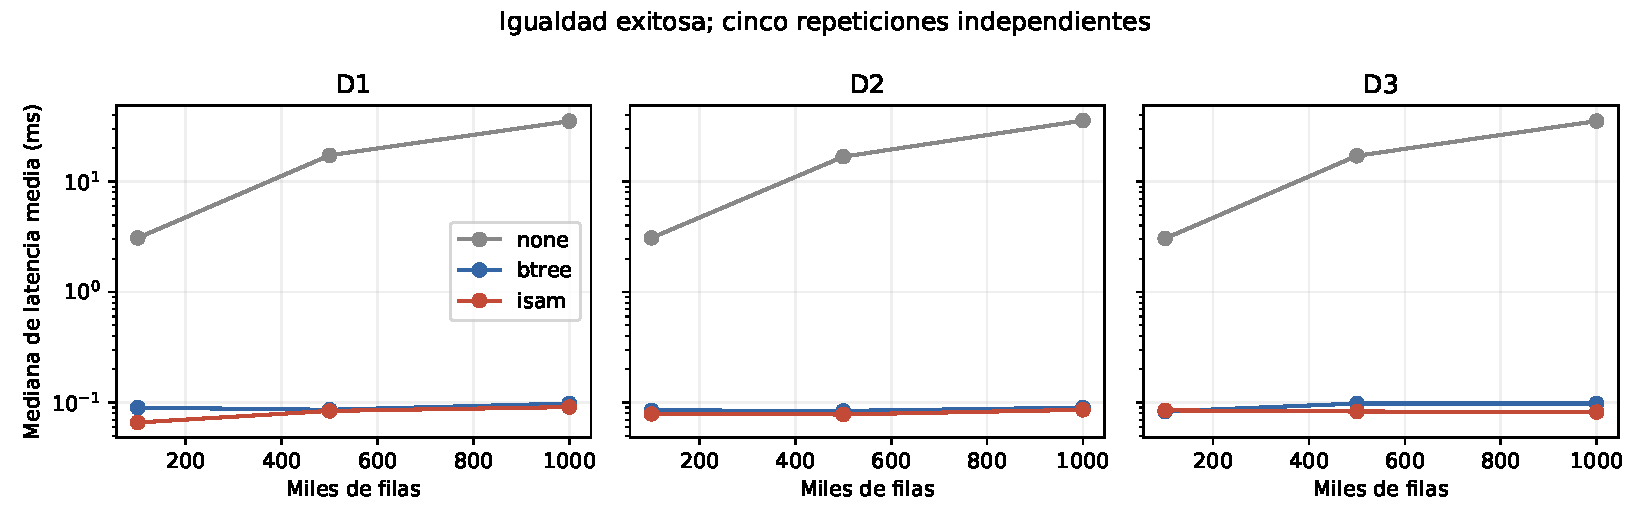
\includegraphics[width=\linewidth]{docs/results/figures/igualdad.pdf}\caption{Igualdad exitosa: escalabilidad observada bajo el protocolo registrado.}\end{figure}

\begin{figure}[htbp]\centering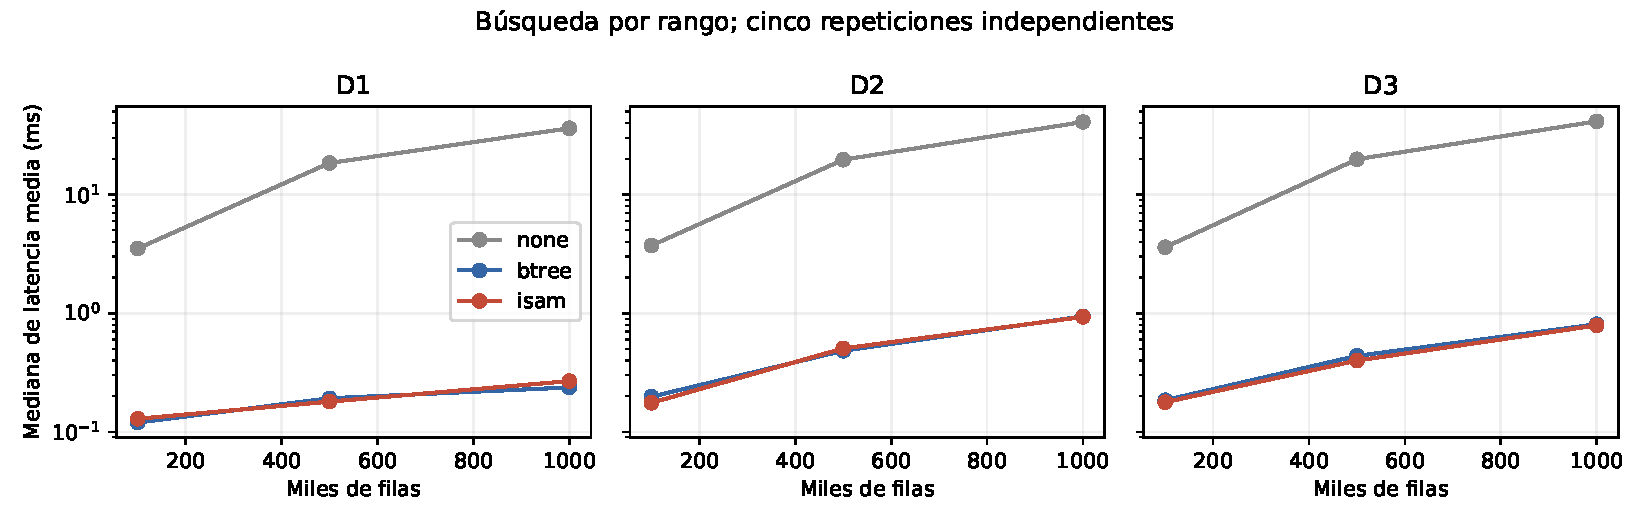
\includegraphics[width=\linewidth]{docs/results/figures/rango.pdf}\caption{Búsqueda por rango: escalabilidad observada bajo el protocolo registrado.}\end{figure}

% END GENERATED BENCHMARK

\subsection{Relleno, concentración y REINDEX}
El experimento adicional carga D1 y concentra lotes de inserciones en una ventana
de 100 claves. Compara B-tree, ISAM con rellenos 60/80/100 y una política ISAM80
con umbral de 25\%. Cada trayectoria se recarga y repite cinco veces. Las lecturas
calientes usan cuotas y semillas fijas. REINDEX vuelve a fijar el relleno de la
configuración para no cambiarlo silenciosamente entre sesiones. La política se
ejecuta desde el runner; su costo y pausas son parte del compromiso de mantenimiento.

Este experimento adicional inserta cada lote mediante un INSERT SELECT en una
transacción. Sus tiempos de inserción por lote no son directamente comparables
con el TPS por transacción de W3; ambos protocolos se identifican por separado.

% BEGIN GENERATED OVERFLOW
Overflow adicional: N inicial = 100000, 5 trayectorias independientes por configuración, 6 lotes de 20000 filas y 1000 consultas calientes por punto.

\begin{table}[htbp]
\centering\small
\caption{Lectura caliente inicial, final y después de REINDEX: mediana [IQR].}\label{tab:overflow}
\resizebox{\linewidth}{!}{%
\begin{tabular}{lrrrrr}
\toprule
Configuración & Inicial ms & Final ms & Cadena final & Tras REINDEX ms & REINDEX ms \\
\midrule
btree & 0.054 [0.006] & 0.531 [0.010] & 0 [0] & 0.504 [0.063] & 63.779 [1.664] \\
isam60 & 0.053 [0.001] & 0.757 [0.034] & 110 [1] & 0.521 [0.099] & 49.909 [3.797] \\
isam80 & 0.057 [0.006] & 0.980 [0.003] & 177 [0] & 0.547 [0.016] & 48.335 [1.321] \\
isam100 & 0.052 [0.010] & 0.951 [0.023] & 177 [0] & 0.533 [0.036] & 44.606 [0.418] \\
isam80t25 & 0.049 [0.003] & 0.551 [0.024] & 0 [0] & -- & -- \\
\bottomrule
\end{tabular}}
\end{table}

\begin{table}[htbp]
\centering\small
\caption{Costo acumulado por trayectoria (medianas, ms) antes del REINDEX final de comparación.}\label{tab:policy}
\resizebox{\linewidth}{!}{%
\begin{tabular}{lrrrr}
\toprule
Configuración & Inserción & Política REINDEX & Suma de costos & MiB finales \\
\midrule
btree & 178.466 & 0.000 & 178.466 & 2.95 \\
isam60 & 657.916 & 0.000 & 657.916 & 3.32 \\
isam80 & 654.008 & 0.000 & 654.008 & 2.84 \\
isam100 & 661.393 & 0.000 & 661.393 & 2.55 \\
isam80t25 & 859.609 & 182.187 & 1044.330 & 3.19 \\
\bottomrule
\end{tabular}}
\end{table}

Los costos de la política se suman por réplica antes de calcular la mediana. Una latencia final cercana a B-tree no significa regresar a la latencia inicial: las inserciones aumentan la cantidad de resultados. La eliminación de overflow tampoco implica siempre menor tamaño físico.

ISAM80 pasó de una mediana de 0.057 ms a 0.980 ms, con cadena final mediana de 177 páginas. Tras REINDEX registró 0.547 ms: cambio de 44.18\% respecto del estado degradado. La mejora combina eliminación de cadenas y reorganización; la lectura de más filas y páginas del heap persiste.

\begin{figure}[htbp]\centering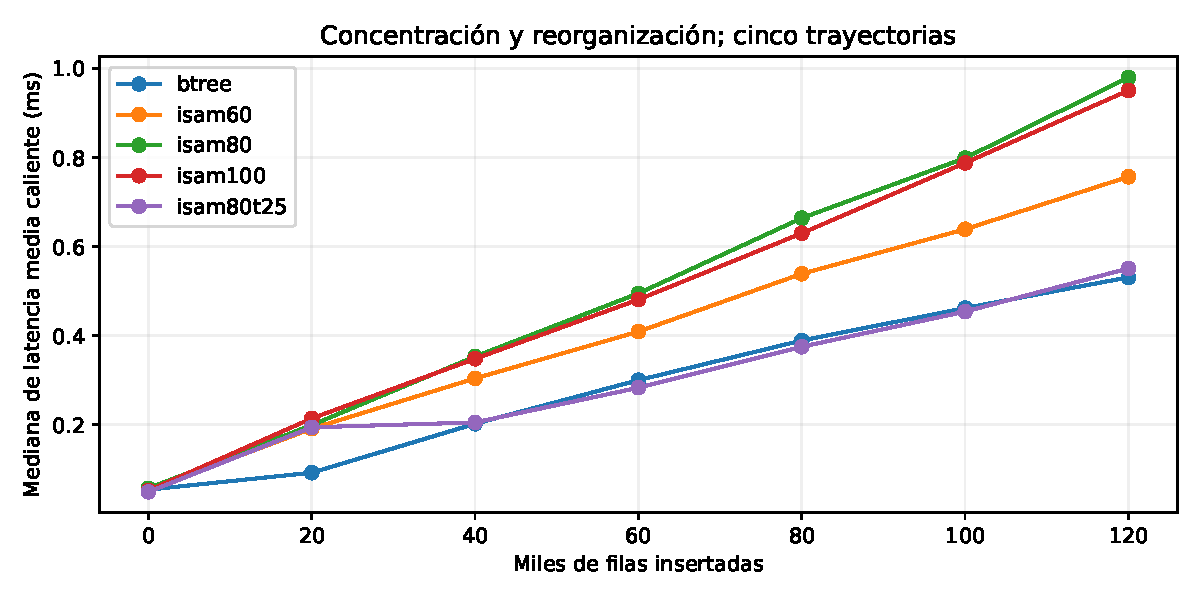
\includegraphics[width=.95\linewidth]{docs/results/figures/overflow.pdf}\caption{Latencia caliente por lote. Los puntos de políticas incluyen el estado posterior a reorganizar.}\end{figure}
\clearpage

% END GENERATED OVERFLOW

No se mezclan aquí los CSV exploratorios anteriores con los corregidos. Esos
CSV tenían D2 con duplicados, D3 con otra distribución y tres repeticiones. La
comparación de espacio bajo duplicados sigue siendo una pregunta útil, pero
debe presentarse como escenario adicional identificado, no como D2 oficial.

\section{Riesgos técnicos y amenazas a la validez}
\begin{longtable}{p{0.27\linewidth}p{0.3\linewidth}p{0.31\linewidth}}
\toprule Riesgo de la propuesta & Impacto & Mitigación aplicada o límite\\\midrule
API interna PostgreSQL & Incompatibilidad y errores de callbacks & Versión 18.6 exacta, PGXS del mismo commit, integración y planes\\
Concentración de overflow & Latencia y crecimiento de cadenas & Métricas SQL, relleno y REINDEX; evaluar también su costo\\
Desarrollo de todas las capas & Complejidad y regresiones & Núcleo separado, pruebas C/SQL y regresión específica de VACUUM\\
Comprensión desigual & Dificultad en defensa individual & Guía, lectura cruzada y ensayo de todas las capas\\
Estado mutable entre réplicas & Comparación injusta & Recarga y construcción independiente; cuotas y huellas\\
Host compartido y cachés & Variabilidad de tiempos & Protocolo explícito, metadatos, mediana e IQR; no afirmar universalidad\\\bottomrule
\end{longtable}

El uso de un tipo int4 y payload de 40 bytes limita la generalización a otras
claves y tamaños de fila. Los rangos pueden devolver cardinalidades diferentes
tras insertar; interpretar el costo del resultado y del heap junto al costo del
índice. La muestra de cinco réplicas satisface el mínimo solicitado, pero no
demuestra equivalencia universal. El host, contenedores y paquetes pueden variar
entre máquinas; la versión fuente y parámetros son verificables, sin prometer
reproducibilidad binaria de todos los paquetes del sistema.

Las alternativas se ejecutan en un orden fijo por réplica. El orden, la actividad
del host y la duración corta de algunas mediciones indexadas pueden introducir
variabilidad; se informa dispersión y no se presentan diferencias pequeñas como
significativas sin análisis estadístico adicional.

La reorganización es total y bloqueante en el flujo probado. No hay búsqueda
index-only, unicidad ni concurrencia completa. El puntero a la cola evita recorrer
la cadena al insertar, pero no reutiliza automáticamente huecos intermedios de
overflow liberados por VACUUM. Las pruebas ante SIGKILL son evidencia de los
casos ejecutados, no una certificación de almacenamiento de producción.

\section{Conclusiones de la Etapa I}
La estructura implementada se utiliza desde PostgreSQL mediante un AM propio,
con construcción, igualdad, rango e inserción en C. La separación de layout,
directorio, escaneo y adaptador del DBMS permite comprobar el mismo núcleo en
standalone y en relaciones reales. La regresión de VACUUM mostró que un mínimo
primario mutable no sustituye un separador estático; su corrección preserva la
fila superviviente y se incorpora a las pruebas de la entrega.

La evaluación corregida distingue valores aleatorios únicos de accesos sesgados
y mantiene cantidades de operaciones iguales. Las conclusiones cuantitativas
deben basarse en las tablas generadas y su dispersión, sin extrapolar cifras de
una máquina a todo contexto. El directorio estático y el overflow explican los
compromisos de ISAM: puede resultar apropiado para datos estables, mientras que
la concentración de inserciones requiere considerar crecimiento de cadenas,
latencia y costo de reconstrucción.

Los bloques 7--8 quedan pendientes. La siguiente etapa debe justificar
fragmentación, asignación y replicación en tres nodos, y evaluar consultas,
latencias, indisponibilidad y cambios de concentración conforme a la rúbrica.
Esta entrega no reclama resultados distribuidos ni una calificación automática
del 100\%; la comprensión y defensa individual deben demostrarse ante la docente.

\section*{Contribución propia y recursos utilizados}
\addcontentsline{toc}{section}{Contribución propia y recursos utilizados}
Según la propuesta, el equipo desarrolla el layout ISAM, directorio, overflow,
callbacks, generadores y harness. Se utilizan PostgreSQL y su interfaz oficial,
GenericXLog, buffer manager, libc, GCC, make, Docker, Python, matplotlib y LaTeX.
La propuesta identifica contrib/bloom y access/heap como referencias de
convenciones, sin atribuirles el núcleo ISAM del proyecto.

Las correcciones, automatización y redacción de esta entrega recibieron asistencia
de OpenAI Codex. Corresponde al equipo revisar, adaptar y comprender el código y
el documento antes de sustentarlos. No se presenta esa asistencia como prueba
de autoría individual ni se inventa una aprobación de la propuesta.

\appendix
\section{Correspondencia con la propuesta inicial, sección 5.5}
\begin{longtable}{p{0.35\linewidth}p{0.53\linewidth}}
\toprule Elemento requerido & Evidencia en esta entrega\\\midrule
Elección y motivación & Introducción; ISAM e igualdad/rango\\
Fuentes de calidad & Bibliografía académica y manual oficial citados en la propuesta\\
Representación y operaciones & Layout y construcción/búsqueda/inserción\\
Clave y consultas & int4, una columna, igualdad y rango\\
Integración PostgreSQL & IndexAmRoutine, opclass y callbacks\\
Componentes del equipo & Núcleo, adaptadores, generadores y harness identificados\\
Recursos externos & Declaración anterior y referencias de la propuesta\\
Riesgos y plan & Matriz de riesgos, semanas S1--S5 y bloques internos 0--6\\\bottomrule
\end{longtable}
La propuesta original de dos páginas se conserva en \code{docs/propuesta-inicial.pdf}.
Este informe amplía la explicación técnica y los resultados; no sustituye ni
pretende cumplir el límite de dos páginas del documento de Semana 1.

\section{Comandos reproducibles y defensa}
\begin{lstlisting}[language=bash]
make test
make integration
make crash
make crash-load
make bench       # 100k, 500k, 1M; D1/D2/D3; 5 replicas
make overflow    # experimento adicional de concentracion
make demo
make pdf
\end{lstlisting}
Las bases de benchmark y overflow son distintas de bd2. Los scripts no borran
volúmenes al arrancar. Las ejecuciones oficiales y sus logs se conservan en
\code{docs/results/}; la guía y preguntas de defensa están en
\code{docs/defensa.md}. Un clon debe incluir estas correcciones; los cambios de
la entrega local no se han subido automáticamente al remoto.

Repositorio: \url{https://github.com/lMafa1813l/BD2-Gestor-isam-postgres}.
\begin{thebibliography}{9}
\bibitem{ramakrishnan} R. Ramakrishnan y J. Gehrke.
\textit{Database Management Systems}, 3.ª edición. McGraw-Hill, 2003.
Capítulos 8 y 10 citados en la propuesta inicial.
\bibitem{silberschatz} A. Silberschatz, H. F. Korth y S. Sudarshan.
\textit{Database System Concepts}. McGraw-Hill. Referencia de estructuras de
indexación citada en la propuesta, que no especifica edición ni páginas.
\bibitem{postgres} PostgreSQL Global Development Group.
\textit{PostgreSQL 18 Documentation: Index Access Method Interface}.
\url{https://www.postgresql.org/docs/18/indexam.html}.
\bibitem{propuesta} Grupo 9, Bases de Datos II.
\textit{Propuesta Inicial -- Proyecto BD II}. Documento entregado por el equipo,
2026. Copia en \code{docs/propuesta-inicial.pdf}.
\bibitem{rubrica} CS272, Bases de Datos II, 2026-II.
\textit{Proyecto BDII: Indexación y Distribución de Datos en PostgreSQL}.
Pautas oficiales aportadas por el equipo, secciones 5--11.
\end{thebibliography}
\end{document}
